
\begin{figure}[ht]
\begin{center}
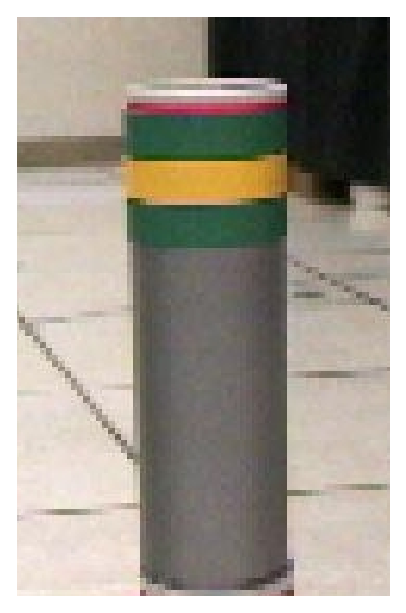
\epsfig{file=laservisualbeacon.eps, height=40mm}
\caption{A sample laser bar (ignore the colored bands).}
\label{fig:laserbar}
\end{center}
\end{figure}

\subsection*{Synopsis}

The laser bar detector searches for retro-reflective targets in the
laser range finder data.  Targets can be either planar or cylindrical,
as shown in Figure \ref{fig:laserbar}.  For planar targets, the range,
bearing and orientation will be determined; for cylindrical targets,
only the range and bearing will be determined.  The target size and
shape can be set in the configuration file.

The range at which targets can be detected is dependant on the target
size, the angular resolution of the laser and the quality of the
retro-reflective material used on the target.

See also the {\tt laserbarcode} and {\tt laservisualbarcode} drivers.

\subsection*{Interfaces}

\noindent Supported interfaces:
\begin{itemize}
\item {\tt fiducial}
\end{itemize}

\noindent Required devices:
\begin{itemize}
\item {\tt laser}
\end{itemize}

\noindent Supported configuration requests:
\begin{itemize}
\item \verb+PLAYER_FIDUCIAL_GET_GEOM+
\end{itemize}


\subsection*{Configuration file options}

\begin{center}
{\small \begin{tabularx}{\columnwidth}{|l|l|c|X|}
\hline
Name & Type & Default & Meaning\\
\hline
{\tt laser} & integer & 0 & Index of the {\tt laser} device to be used. \\
{\tt shape} & string & ``cylinder'' & Target shape: ``plane'' or ``cylinder''. 
Planar fiducials are currently not supported.\\
{\tt width} & length & 0.08 & Target width (m). \\
\hline
\end{tabularx}}
\end{center}

\subsection*{Notes}
